\chapter{洗浄後に掌へ残存するウイルス量に基づく感染リスク評価}

本章では、第6章までに得られた水分付着量および洗浄後の掌へのウイルス残存率に関する実験結果を基に、
洗浄後に手指へ残存するウイルスによる感染リスクを定量的に評価することを目的とする。前章までの検討により、
水分付着量およびウイルス残存率は個人差や左右差の影響を受けにくく、一般化可能な確率分布としてモデル化できることが示された。
そこで本研究では、これらの分布を用い、汚染された河川水に手が接触した場合を想定した微生物定量的リスク評価（QMRA）を実施し、
モンテカルロシミュレーションにより感染リスクを予測した。

\section{QMRAの概要}

QMRA（Quantitative Microbial Risk Assessment：微生物定量的リスク評価）は、
病原微生物に曝露した場合にどの程度感染が生じる可能性があるかを、科学的根拠に基づいて数値的に推定する手法である。
QMRAを用いることで、洗浄や消毒の効果を「効果がある・ない」といった定性的な評価ではなく、感染確率という定量的な指標として
評価することが可能となる。

QMRAは、食品衛生、飲料水の安全管理、院内感染対策、下水・環境衛生分野などにおいて広く用いられており、
衛生管理の最適化に寄与する重要な評価手法である。例えば、ある表面に10,000個のウイルスが付着している状況で洗浄を行い、
100個まで減少した場合、除去率99\%と定量的に示すことができる。
このように、QMRAは洗浄・消毒操作が感染リスクをどの程度低減するかを明確に示す上で有効である。

また、QMRAでは「曝露量 → 宿主体内への侵入量 → 感染成立」という感染成立の過程をモデル化する。
特にノロウイルスのように感染力の強いウイルスでは、ごく少量の曝露でも感染が成立する可能性があるため、
微量レベルでの曝露評価が重要となる。本章では、QMRAの考え方を用いて、
手指に付着した汚染水中のウイルスが洗浄条件の違いによってどの程度感染リスクに影響するかを評価する。

\section{リスクシナリオの設定}

本研究では、河川水に下水処理水が混入した状況を想定し、その水が手指に付着した場合の感染リスクを評価対象とした。
対象とする病原体はノロウイルスとし、前章までに得られた「洗浄後のMS2残存率モデル」および「手指への水分付着量の確率分布」
を統合したリスク評価シナリオを設定した。
曝露頻度については、短期間における集中的な利用を想定し、
1か月間にわたり毎日1回、汚染水に手指が接触する状況を評価対象とした。
すなわち、本研究では曝露イベント数を30回と設定し、短期間における累積感染リスクの評価を行った。

\subsection{想定する感染経路}

本研究で想定した感染経路を以下に示す。

\begin{enumerate}
  \item 汚染された河川水が手指（掌全体）に付着する。
  \item 洗浄操作を行う（0回～5回、100\,mL/回）。
  \item 洗浄後に掌へ残存したウイルスの一部が手から口へ移行する。
  \item 経口摂取されたウイルス量に基づき、容量反応モデルを用いて感染成立確率を算定する。
\end{enumerate}

\subsection{評価ケースの設定}

本研究では、第6章の統計解析結果を踏まえ、以下の3つの洗浄条件を評価ケースとして設定した。

\begin{itemize}
  \item Case 0：洗浄なし
  \item Case 1：洗浄1回（100\,mL）
  \item Case 2：洗浄2～5回（分割洗浄）
\end{itemize}

第6章の多重比較結果より、洗浄2回目以降ではウイルス残存率に有意な差が認められなかったことから、
本研究では洗浄2～5回の条件を1つの群として統合して取り扱った。

\section{感染リスク評価に用いた計算ロジック}

本研究では、洗浄後に掌へ残存するウイルス量を基に感染リスクを評価するため、
確率論的な計算モデルを構築した。
本節では、図\ref{fig:qmra_flow} に示した QMRA の流れに沿って、
モンテカルロシミュレーションに用いた計算ロジックについて説明する。

\begin{figure}[t]
  \centering
  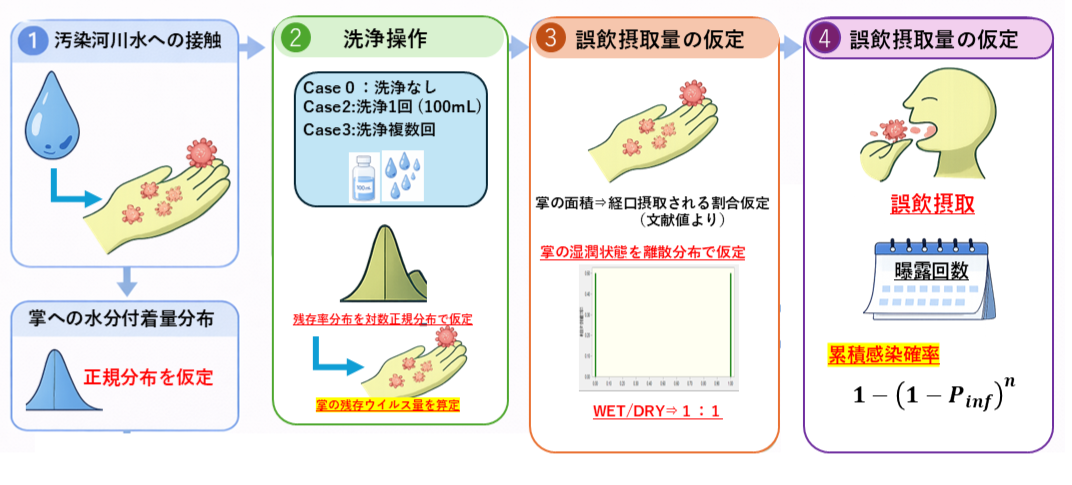
\includegraphics[width=0.95\linewidth]{fig/QMRA_Procedure.png}
  \caption{本研究におけるQMRAに基づく感染リスク評価の計算フロー}
  \label{fig:qmra_flow}
\end{figure}


\subsection{初期付着ウイルス量の算出}

まず、汚染水に手指が接触した際に掌へ付着する初期ウイルス量を算出した。
図\ref{fig:qmra_flow} の①に示すように、
下水処理水が混入した河川水に掌全体が接触する状況を想定した。

河川水中のノロウイルス濃度については、
既報の文献値を基に対数正規分布(図\ref{fig:logdist_river})を仮定し、
モンテカルロシミュレーションの各試行ごとにランダムにサンプリングした。
一方、手指に付着する水分量については、
第3章で得られた実験結果に基づき水分付着量分布の正規分布を仮定した。

\begin{figure}[t]
  \centering
  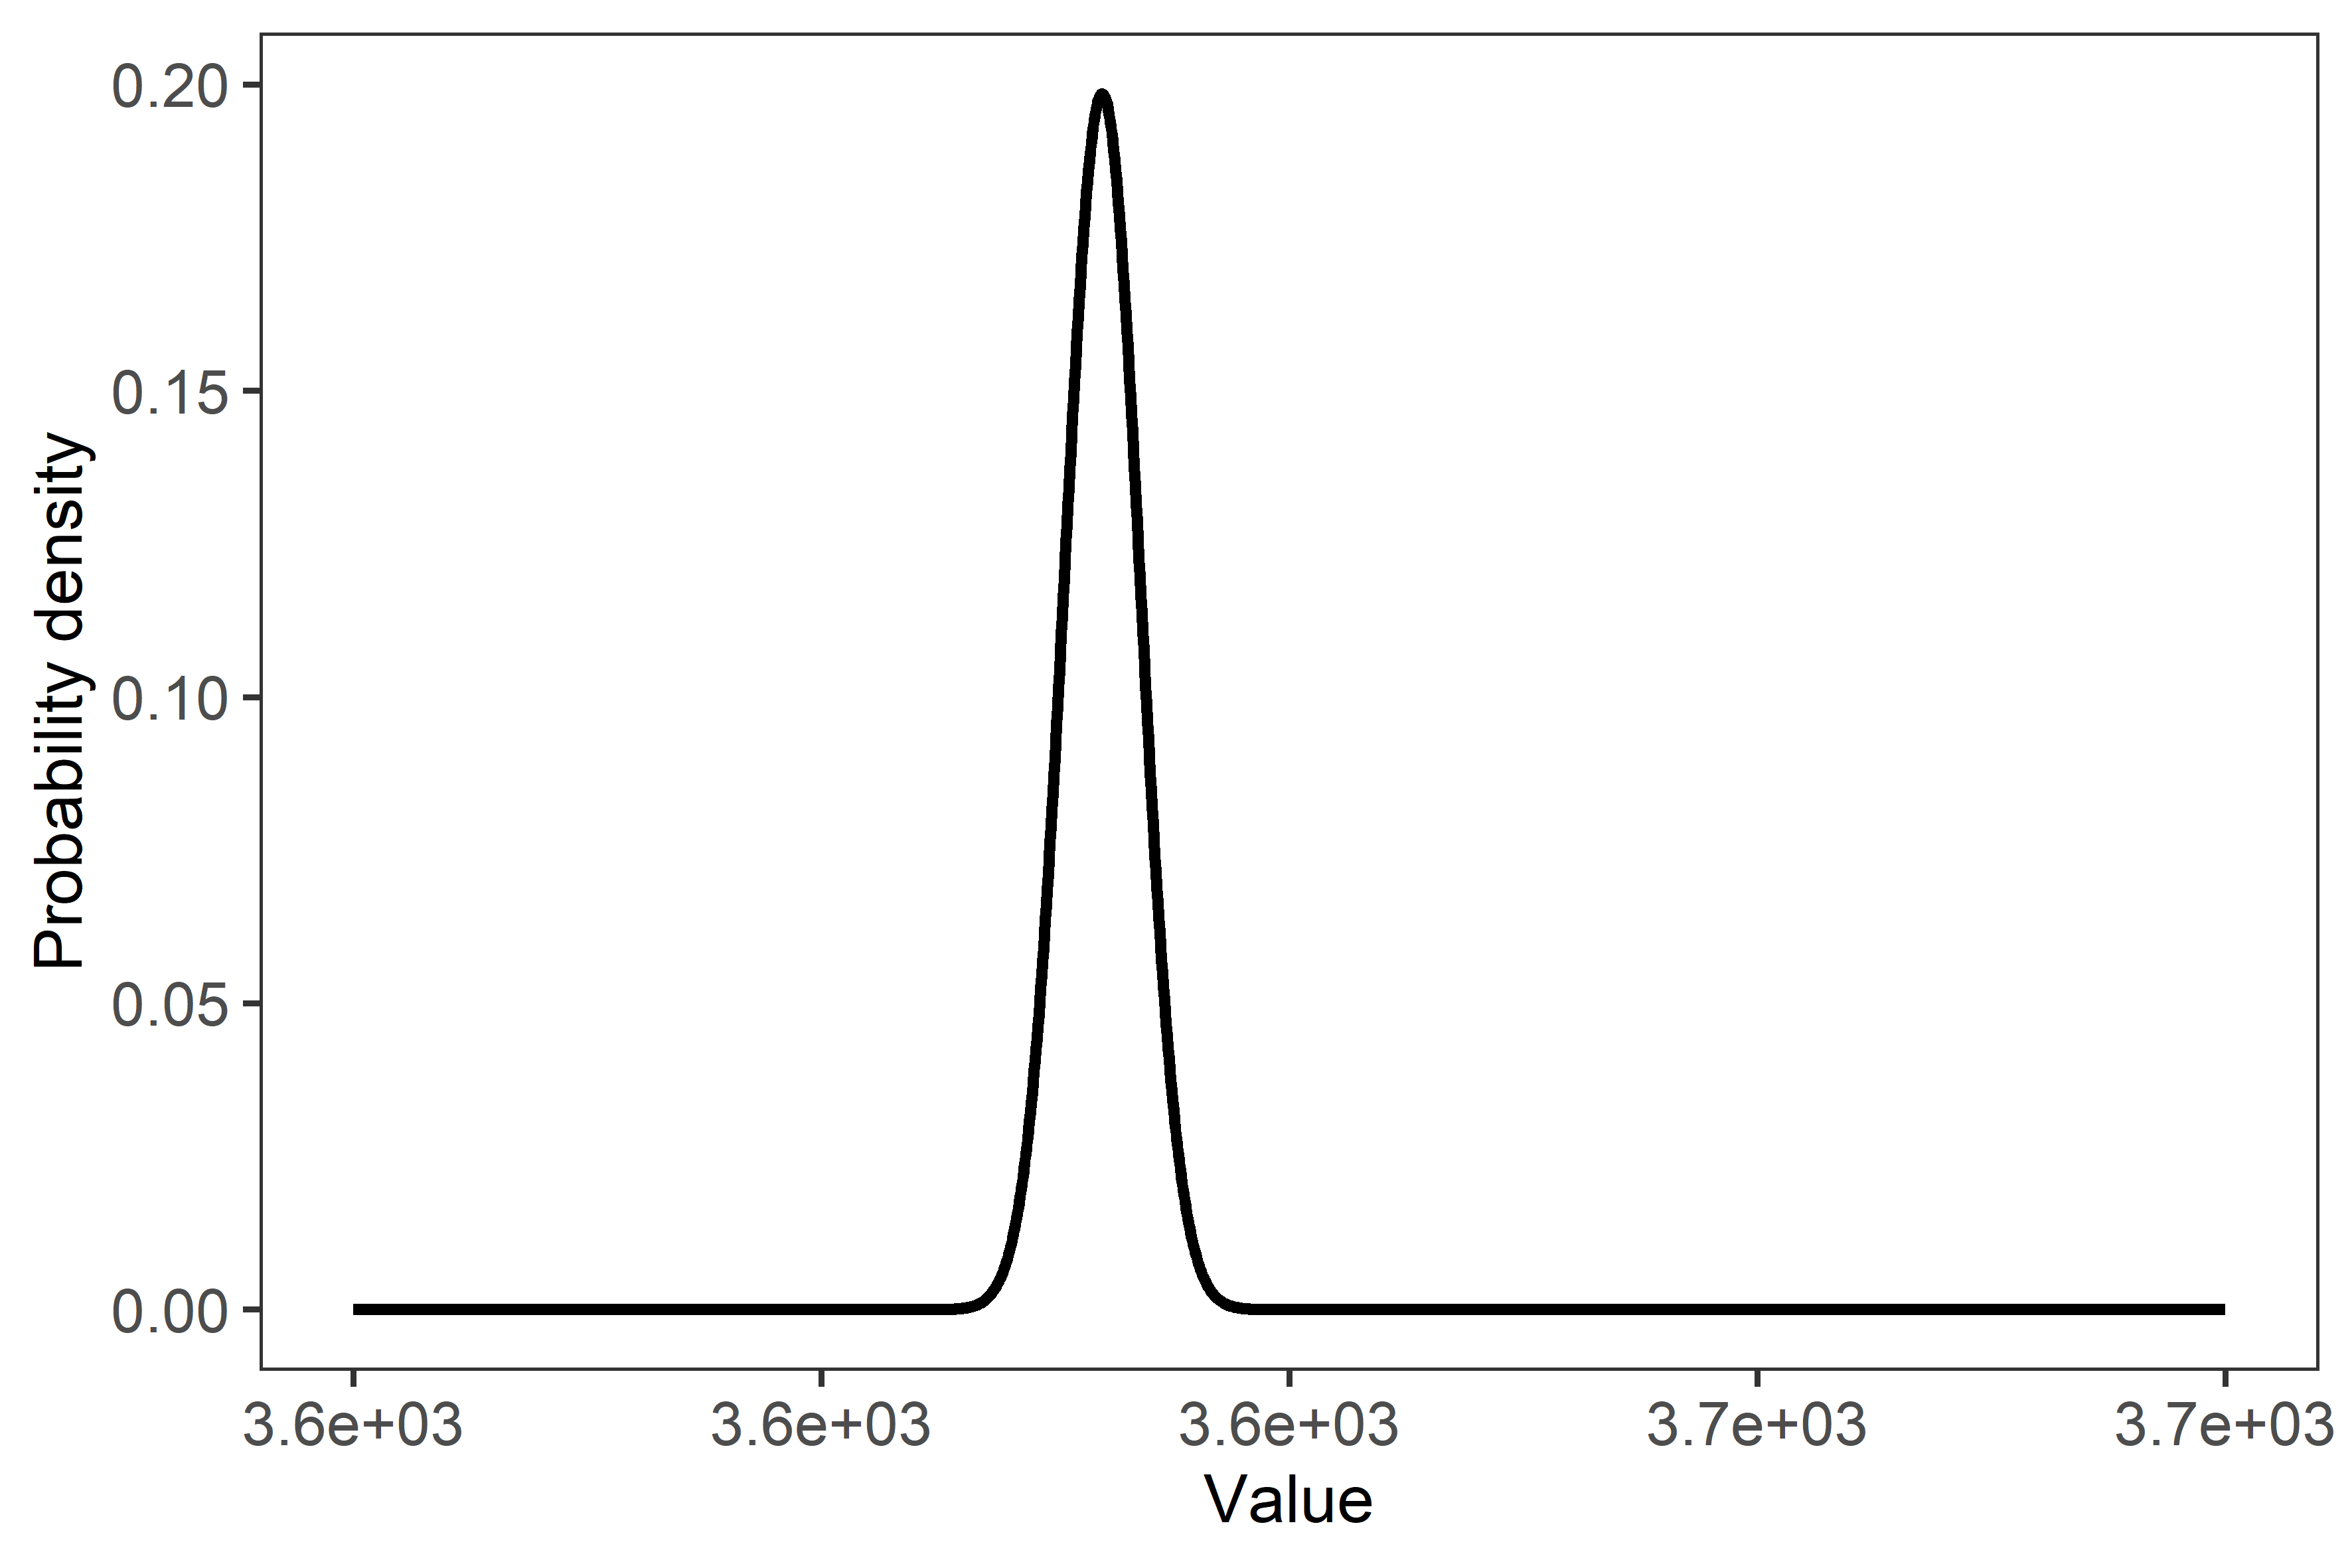
\includegraphics[width=0.75\linewidth]{fig/river_dist.png}
  \caption{河川水中のウイルス濃度の対数正規分布モデル（文献値に基づく）}
  \label{fig:logdist_river}
\end{figure}

これらより、掌に付着する初期ウイルス量 $N_0$ は、
以下の式により算出した。

\begin{equation}
N_0 = C_{\mathrm{river}} \times W
\end{equation}

ここで、$C_{\mathrm{river}}$ は河川水中のノロウイルス濃度（対数正規分布）、
$W$ は手指に付着した水量（正規分布）である。

\subsection{洗浄後の掌残存ウイルス量}

次に、洗浄操作によるウイルス除去効果を考慮した。
図\ref{fig:qmra_flow} の②に示すように、
洗浄条件として洗浄なし、洗浄1回（100 mL）、
および洗浄2～5回（分割洗浄）の条件を設定した。

洗浄後に掌へ残存するウイルス量は、
初期付着ウイルス量に洗浄条件ごとの残存率を乗じることで算出した。
洗浄1回目および洗浄2～5回目の残存率については、
第6章の解析結果を基に、
いずれも対数正規分布としてモデル化した。
洗浄なしの場合については、
残存率を1と仮定した。

洗浄後の掌残存ウイルス量 $N_{\mathrm{hand}}$ は、
以下の式で表される。

\begin{equation}
N_{\mathrm{hand}} = N_0 \times R
\end{equation}

ここで、$R$ は洗浄条件に応じたウイルス残存率である。

\subsection{手から口への誤飲摂取割合}

洗浄後に掌へ残存したウイルスのすべてが感染に寄与するわけではないため、
本研究では手から口への誤飲摂取割合を考慮した。
図\ref{fig:qmra_flow} の③に示すように、
誤飲摂取割合は、
口に接触する手指面積の割合と、
手指表面から口腔内へのウイルス移行率の積として表現した。

口に接触する面積割合および移行率については、
いずれも文献値を基に Beta 分布を仮定した。
また、手指の状態を乾燥状態（dry）および湿潤状態（wet）の
2 状態に分類し、
それぞれが同程度の確率（50\%）で生じると仮定した。
各試行において、
手指の状態をランダムに決定し、
対応する移行率を適用することで、
誤飲摂取割合を算出した。

\subsection{経口摂取量および感染確率の算出}

経口摂取量 $D$ は、
洗浄後に掌へ残存するウイルス量と、
手から口への誤飲摂取割合の積として算出した。

\begin{equation}
D = N_{\mathrm{hand}} \times f_{\mathrm{ing}}
\end{equation}

ここで、$f_{\mathrm{ing}}$ は誤飲摂取割合であり、
洗浄後に掌へ残存したウイルスのうち、
経口的に体内へ取り込まれる割合を表す。

本研究では、誤飲摂取割合を、
(1) 口に接触する手指（掌）の面積割合と、
(2) 手指表面から口腔内へのウイルス移行率の積としてモデル化した。
これらはいずれも 0 から 1 の範囲に制約される割合であり、
個人差や状況によって変動するため、
確率分布として扱うことが妥当であると考えられる。
そこで、口に接触する面積割合および移行率については、
文献値を基に Beta 分布を仮定した。

また、手指表面の状態によって、
ウイルスの移行率が異なることが報告されている。
特に、手指が湿潤状態（wet）の場合には、
乾燥状態（dry）と比較して、
手から口へのウイルス移行が起こりやすいとされている。
そのため本研究では、
移行率を $TE_{\mathrm{dry}}$ および $TE_{\mathrm{wet}}$ に分け、
それぞれを Beta 分布として設定した。
さらに、日常的な状況を想定し、
手指の状態は dry と wet が同程度の確率で生じると仮定し
（50\%, 50\%）、
各試行においていずれかの状態をランダムに選択する
混合分布として移行率を決定した。

以上の方法により、
洗浄後に掌へ残存するウイルス量から、
経口摂取量 $D$ を確率論的に算出した。
なお、本研究では、
指標ウイルスとして用いた MS2 ファージの残存挙動が、
ノロウイルスの挙動を代表できるものと仮定し、
MS2 ファージの残存率を
ノロウイルスにも適用した。

感染確率の算出には、
ノロウイルスの容量反応モデルを用い、
ID$_{50}$ を 10 および 100 とする
2 条件を設定した。
まず、1 回の曝露における感染確率を算出し、
その後、
1 か月間に毎日 1 回曝露する状況を想定して、
曝露回数を $n=30$ とした場合の
累積感染確率を算出した。


\section{モンテカルロシミュレーションの実施}

以上の計算ロジックに基づき、
Crystal Ball を用いて 10,000 回の
モンテカルロシミュレーションを実施した。
各試行において、
河川水中のノロウイルス濃度、
手指に付着する水分量、
洗浄後のウイルス残存率、
および誤飲摂取割合を
それぞれの確率分布からランダムにサンプリングし、
洗浄条件別に感染確率を算出した。

次節では、
これらのシミュレーション結果を基に、
洗浄条件の違いによる感染リスクの比較および考察を行う。

\section{モンテカルロシミュレーション結果}

前節で示した計算ロジックに基づき、
Crystal Ball を用いて10,000回のモンテカルロシミュレーションを実施した。
洗浄条件として、
Case0（洗浄なし）、
Case1（洗浄1回、100 mL）、
Case2（洗浄複数回）
の3条件を設定し、
曝露回数を1か月間に毎日1回とした30回の累積曝露として、
累積感染確率を算出した。

シミュレーションの結果を図\ref{fig:infection_risk} に示す。
各洗浄条件における累積感染確率は、
単一の値ではなく幅をもった分布として得られた。
そこで本研究では、
感染リスクの代表値および分布の広がりを把握するため、
5\%タイル値、
中央値（50\%タイル値）、
95\%タイル値を指標として結果を整理した。

\begin{figure}[p]
  \centering
  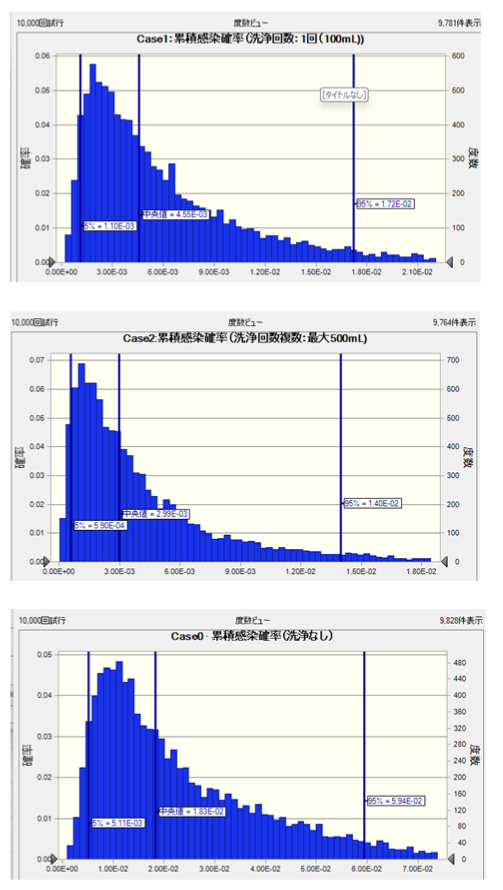
\includegraphics[width=0.75\linewidth]{fig/infection probability.png}
  \caption{各Caseに基づく累積感染確率分布の比較}
  \label{fig:infection_risk}
\end{figure}

\clearpage

Case0（洗浄なし）では、
累積感染確率の5\%タイル値は
$5.26\times10^{-3}$、
中央値は
$1.82\times10^{-2}$、
95\%タイル値は
$5.90\times10^{-2}$
であった。
これは、
比較的条件が良い場合でも
約0.5\%程度の感染リスクが存在し、
条件が重なった場合には
数\%オーダーの感染リスクに達する可能性があることを示している。

Case1（洗浄1回、100 mL）では、
5\%タイル値が
$1.13\times10^{-3}$、
中央値が
$4.62\times10^{-3}$、
95\%タイル値が
$1.77\times10^{-2}$
となった。
洗浄を1回行うことで、
洗浄なしの場合と比較して、
中央値および高リスク側の値が
全体として低下しており、
単回洗浄であっても
感染リスク低減に一定の効果があることが示された。

Case2（洗浄複数回）では、
5\%タイル値が
$6.27\times10^{-3}$、
中央値が
$2.94\times10^{-3}$、
95\%タイル値が
$1.37\times10^{-2}$
であった。
中央値および95\%タイル値に着目すると、
洗浄1回の場合と同程度、
あるいはやや低い値を示しており、
複数回洗浄によって
感染リスクがさらに低下する傾向が確認された。
一方で、
5\%タイル値では
洗浄1回の場合よりも大きな値を示しており、
条件によっては
複数回洗浄を行っても
一定の感染リスクが残存する可能性が示された。

これらの結果は、
感染リスクが常に同じ値になるのではなく、
河川水中のウイルス濃度、
手指に付着する水分量、
洗浄後に残るウイルス量、
および手から口へ移行する割合といった要因が、
状況ごとに変化することによって、
ばらつきをもって現れることを示している。
本研究では、
このようなばらつきを考慮するため、
感染リスクを分布として評価した。
中央値は、
平均的な条件を想定した場合の
代表的な感染リスクを示す値であり、
95\%タイル値は、
条件が重なった場合を想定した、
やや厳しい状況下での
感染リスクを示す指標として解釈できる。

\section{考察}

本研究で得られた結果から、
洗浄操作は、
汚染水への接触後に生じる感染リスクを
低減する上で有効であることが示された。
特に、
洗浄なしの場合と比較すると、
洗浄を1回行うだけでも、
累積感染確率の中央値および
高リスク側の値が大きく低下しており、
初回の洗浄が感染リスク低減において
重要な役割を果たしていることが示唆された。

一方で、
洗浄回数を増やした場合でも、
感染リスクが完全にゼロになるわけではなく、
一定の確率でリスクが残存することが明らかとなった。
これは、
河川水中のウイルス濃度や
誤飲摂取割合などが
条件によって大きく変動するためであり、
洗浄操作のみで
すべての感染リスクを排除することが
困難であることを示している。

また、
Case1（洗浄1回）と
Case2（洗浄複数回）の結果を比較すると、
中央値および95\%タイル値では
大きな差は認められなかった。
この傾向は、
第6章で示した
「初回洗浄でウイルスの大部分が除去され、
2回目以降の洗浄による追加効果は限定的である」
という実験結果と整合している。

以上より、
本研究のシナリオ条件下では、
洗浄回数を過度に増やすよりも、
確実に初回の洗浄を行うことが
感染リスク低減において
重要であると考えられる。
本研究で用いたQMRA手法は、
洗浄操作の効果を
確率論的に評価する枠組みとして有用であり、
今後、
異なる曝露頻度や洗浄条件を想定した評価にも
応用可能であると考えられる。

\enlargethispage{1\baselineskip}